\documentclass[11pt,a4paper]{article}
\usepackage[utf8]{inputenc}
\usepackage[T1]{fontenc}
\usepackage{lmodern}
\usepackage[french]{babel}
\usepackage[margin=2.1cm]{geometry}
\usepackage{microtype}
\usepackage{amsmath,amssymb}
\usepackage{booktabs}
\usepackage{array}
\usepackage[table]{xcolor}
\usepackage{graphicx}
\usepackage{caption}
\usepackage[most]{tcolorbox}
\definecolor{navy}{HTML}{1F3864}
\definecolor{bluemid}{HTML}{2E5496}
\definecolor{lightblue}{HTML}{D6E0F0}
\captionsetup{font=small,labelfont={bf,color=navy},labelsep=period}
\graphicspath{{../figures/}}
\newtcolorbox{cle}[1][]{colback=lightblue!40,colframe=navy,boxrule=0.6pt,
  arc=2pt,left=8pt,right=8pt,top=6pt,bottom=6pt,#1}

\title{\vspace{-1.2cm}\color{navy}\bfseries Le sous-process tiers (P4) sur donnée ouverte\\[2pt]
  \large Ce qu'on peut ancrer avant le registre de Mehdi}
\author{Kélian Kaddouri}
\date{27 juillet 2026}

\begin{document}
\maketitle
\vspace{-0.9cm}

\begin{cle}
\textbf{La question.} Descendre P4 (risque tiers) au niveau \emph{sous-process} suppose le
registre d'externalisation DORA (structure fixée par l'ITS 2024/2956, à fournir par l'entité).
En attendant, que dit déjà la donnée ouverte ? Réponse en deux temps opposés : la taxonomie fine
est rare, mais l'origination et la concentration sont ancrées sur donnée européenne officielle.
\end{cle}

\medskip
\begin{center}
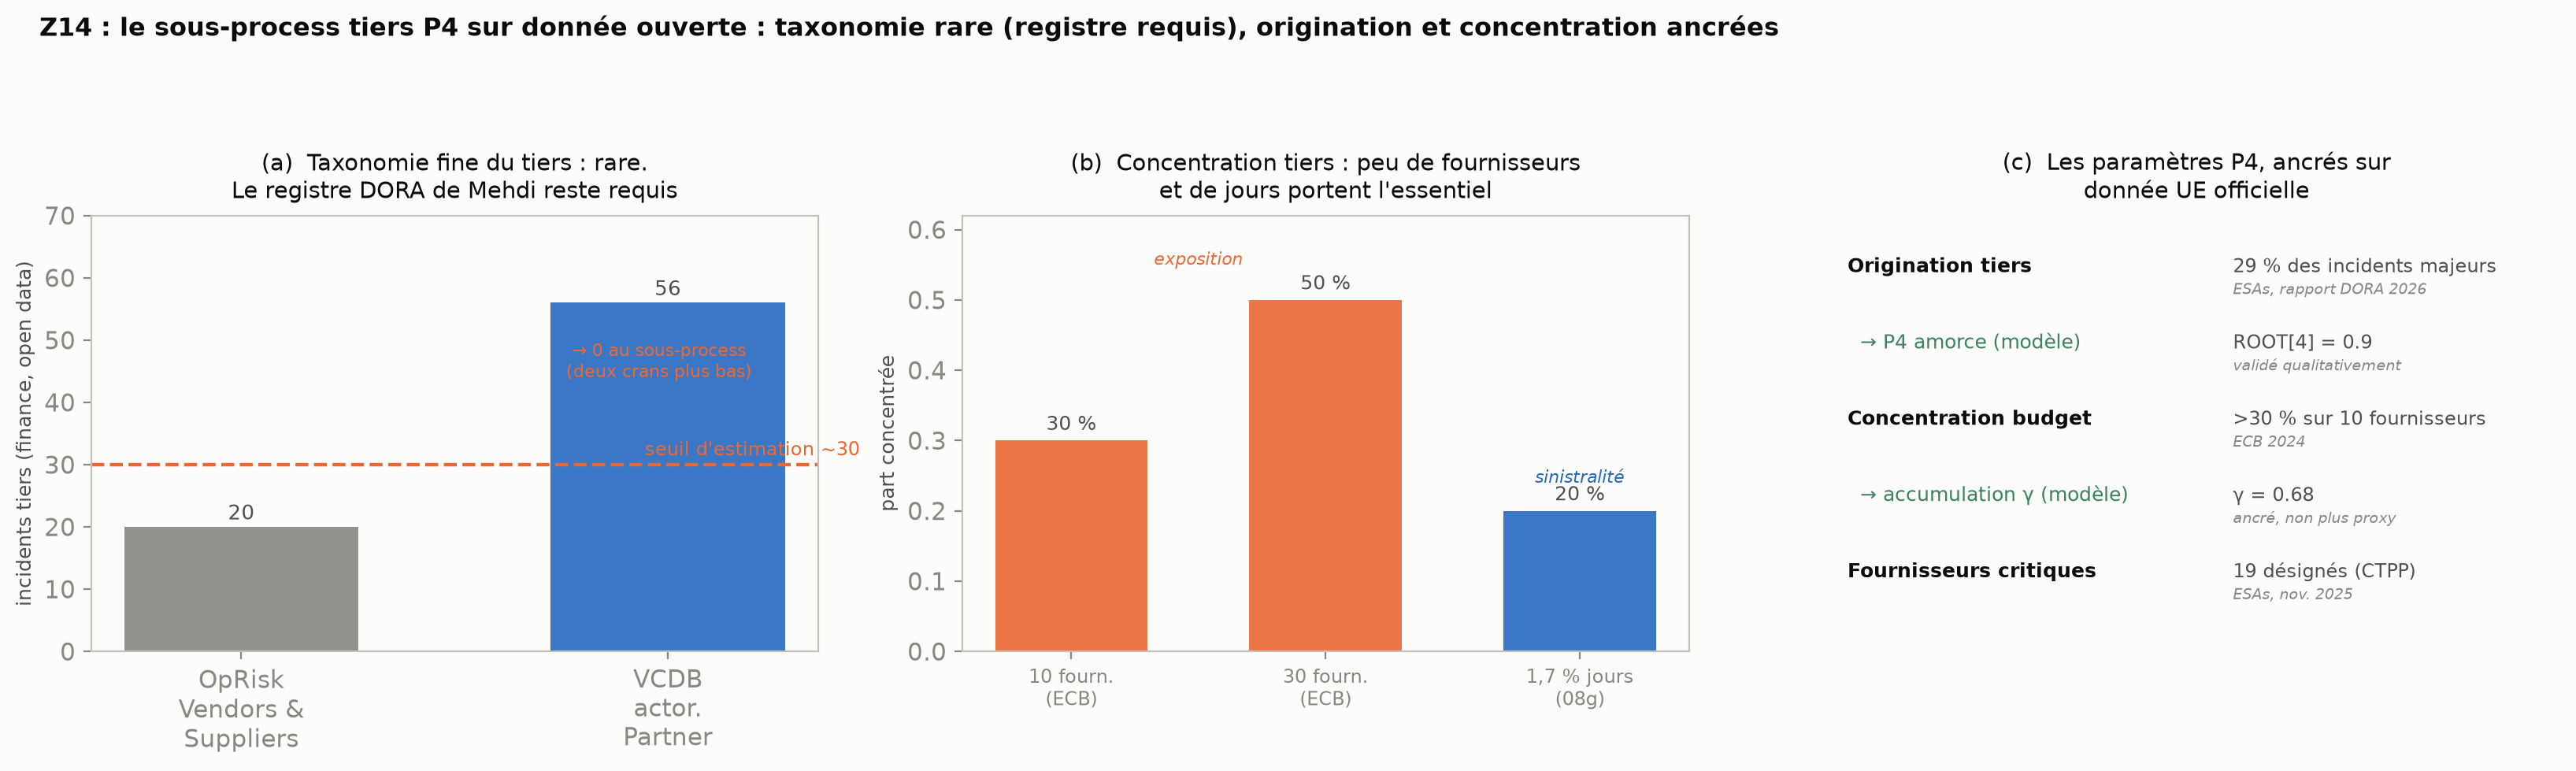
\includegraphics[width=\linewidth]{Z14_p4_sousprocess_open.png}
\captionof{figure}{\textbf{(a)} la taxonomie fine du tiers est sous le seuil d'estimation (le
registre DORA reste requis). \textbf{(b)} la concentration, elle, est nette, côté exposition
(BCE) comme côté sinistralité (Gini $0{,}69$). \textbf{(c)} origination et concentration tierces
ancrées sur donnée UE officielle.}
\end{center}

\noindent\textbf{(1) La taxonomie fine du tiers est rare partout.} La sous-catégorie
\og{}Vendors \& Suppliers\fg{} d'OpRisk ne compte que $20$ incidents en finance ($1\,\%$ du
TIC), et \texttt{actor.Partner} du VCDB $56$, s'effondrant à zéro deux niveaux plus bas. Le
\emph{qui} (quel sous-traitant, quelle fonction critique, quelle substituabilité) n'est pas
résoluble sur open data : il faut le registre. C'est la thèse \og{}donnée manquante =
spécification de reporting\fg{}, déclinée au sous-process P4.

\medskip
\noindent\textbf{(2) L'origination et la concentration sont ancrées.}
\begin{itemize}\itemsep2pt
\item \textbf{Origination} : le premier rapport d'incidents DORA des ESAs (3~juin 2026) établit
que \textbf{$29\,\%$} des $3\,383$ incidents \textsc{tic} majeurs de $2025$ proviennent d'une
défaillance de \textbf{tiers}. P4 est bien une amorce majeure, ce que le classeur posait par
jugement ($\text{\texttt{ROOT}}[4]=0{,}90$).
\item \textbf{Concentration} : l'analyse des registres par la BCE (2024) montre que plus de
$30\,\%$ du budget d'externalisation des grandes banques va à $10$ fournisseurs ($50\,\%$ du
budget critique à $30$), et les ESAs ont désigné $19$ fournisseurs \textsc{tic} critiques. Cela
\textbf{ancre} le paramètre d'accumulation $\gamma=0{,}68$, jusque-là un proxy cloud.
\end{itemize}

\begin{cle}[colback=orange!8,colframe=orange!70!black]
\textbf{Verdict.} On peut avancer \emph{sans} Mehdi sur la partie identifiée (origination,
accumulation symétrique), désormais adossée à des chiffres UE officiels, et réserver au registre
la seule partie non résoluble (la taxonomie fine des sous-traitants). Quand le registre arrivera,
il se branchera sur des paramètres déjà ancrés plutôt que sur des proxys.
\end{cle}

\smallskip
\noindent\footnotesize\textcolor{navy}{\textbf{Source.}} Script
\texttt{9\_cas\_usage/44\_p4\_sousprocess\_open.py}, figure \texttt{Z14\_p4\_sousprocess\_open.png}.
Ancres : ESAs (rapport incidents DORA 2026), BCE (registres 2023), ESAs (désignation CTPP 2025).

\end{document}
